\documentclass[12pt,letterpaper]{article}
\usepackage{fullpage}
\usepackage[top=2cm, bottom=4.5cm, left=2.5cm, right=2.5cm]{geometry}
\usepackage{amsmath,amsthm,amsfonts,amssymb,amscd}
% \usepackage{lastpage}
\usepackage{enumerate}
\usepackage{fancyhdr}
% \usepackage{mathrsfs}
\usepackage{xcolor}
\usepackage{graphicx}
\usepackage{listings}
\usepackage{hyperref}

% define vector
\newcommand{\q}{\underline}
\newcommand{\mt}{\mathrm}

% define in-line code
\definecolor{codegray}{gray}{0.9}
\newcommand{\code}[1]{\colorbox{codegray}{\texttt{#1}}}

\hypersetup{%
  colorlinks=true,
  linkcolor=blue,
  linkbordercolor={0 0 1}
}

\renewcommand\lstlistingname{Snippet}
\renewcommand\lstlistlistingname{Snippet}
\def\lstlistingautorefname{Snippet.}

\lstdefinestyle{python}{
    language        = python,
    frame           = lines, 
    basicstyle      = \footnotesize,
    keywordstyle    = \color{violet},
    stringstyle     = \color{green},
    commentstyle    = \color{red}\ttfamily
}


\setlength{\parindent}{0.2in}
\setlength{\parskip}{0.1in}

% Edit these as appropriate
\newcommand\course{STAT203A}
\newcommand\hwnumber{1}                  % <-- homework number
\newcommand\NetIDa{M.-F. Ho}           % <-- NetID of person #1
% \newcommand\NetIDb{netid12038}           % <-- NetID of person #2 (Comment this line out for problem sets)

\pagestyle{fancyplain}
\headheight 35pt
\lhead{\NetIDa}
% \lhead{\NetIDa\\\NetIDb}                 % <-- Comment this line out for problem sets (make sure you are person #1)
\chead{\textbf{\Large Homework 3}}
\rhead{\course \\ \today}
\lfoot{}
\cfoot{}
\rfoot{\small\thepage}
\headsep 1.5em

\newcommand{\Data}{\mathcal{D}}
\newcommand{\xvec}{\boldsymbol{x}}
\newcommand{\Xvec}{\boldsymbol{X}}
\newcommand{\Var}{\textrm{Var}}
\newcommand{\normal}{\textrm{N}}
\newcommand{\xmean}{\langle \xvec \rangle}
\newcommand{\newx}{\tilde{x}}
\newcommand{\integer}{\mathbb{N}}
\newcommand{\thetarv}{\tilde{\theta}}
\newcommand{\phirv}{\tilde{\phi}}

\newcommand{\ml}{m_{\ell}}
\newcommand{\specterms}{^{2S+1}\mathcal{L}^p_\mathcal{J}}

\begin{document}

\section*{3.1: SII ion}

The electronic configuration is $1s^2 2s^2 2p^6 3s^2 3p^3$.

So we have three electrons in the shell, we have to guess how many configurations we could possibly rearrange them.
We know that $\ml = -1, 0, 1$ and we know $m_s = -1/2, 1/2$.
We have to distribute 3 electrons into $3\times 2$ slots:
\begin{equation}
    C^{6}_3 = \frac{6 \times 5 \times 4}{3!} = 20.
\end{equation}

I crudely all the possibilities here, based on Pauli exclusion principle:
\begin{figure*}[h]
    \centering
    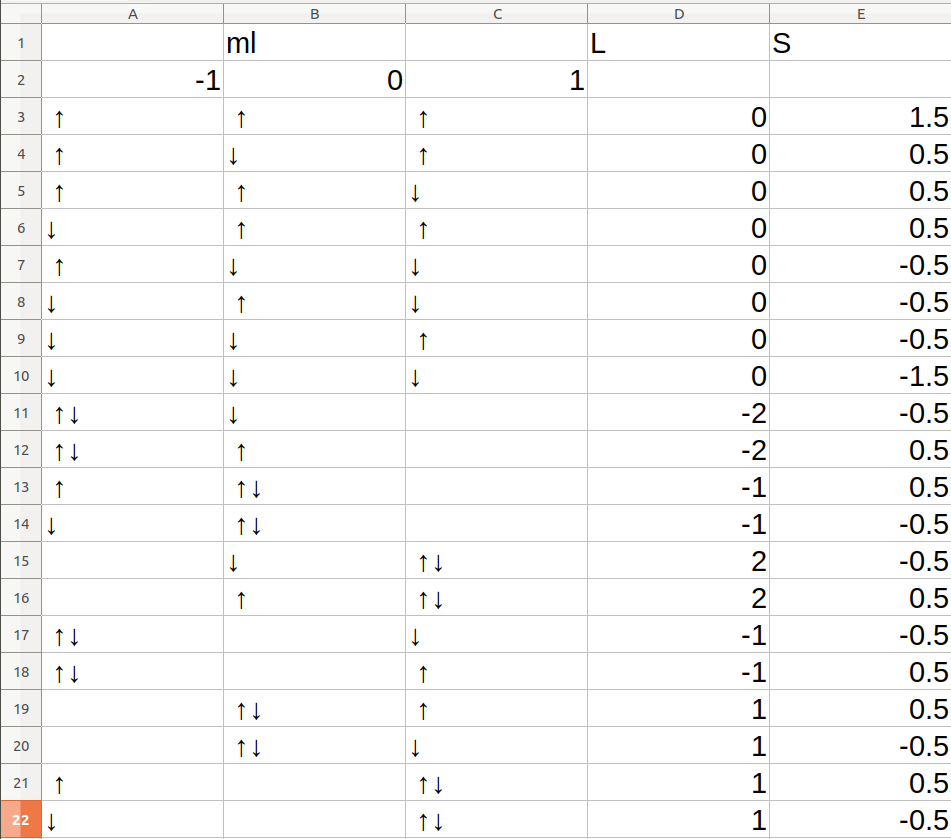
\includegraphics[width=0.75\textwidth]{images/table.png}
    \caption{electron configuration}
    \label{fig:table}    
\end{figure*}

Of course we need to write into spectroscopic terms like:
\begin{equation*}
    \specterms,
\end{equation*}
where $\mathcal{L} \in \{S, P, D, ...\}$ and $p \in \{\mt{odd}, \mt{blank} \}$, and $\mathcal{J} = S + L$.

Now we examine the total spin and total angular momentum in our list, and we get the last 2 columns in Fig~\ref{fig:table}.

We follow the procedure taught in the class, and write these possibilities into a cubic:
\begin{figure}[h]
    \centering
    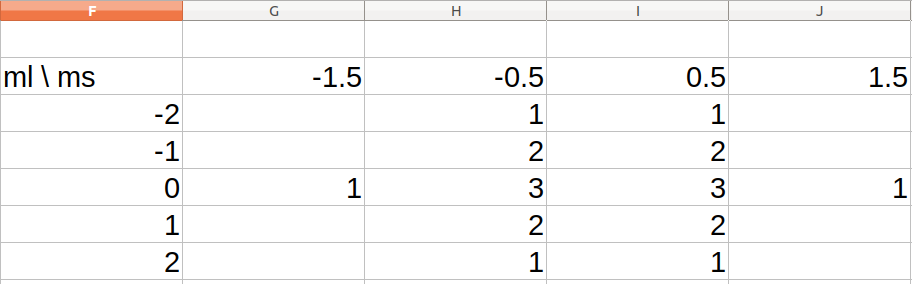
\includegraphics[width=0.75\textwidth]{images/cubic.png}
\end{figure}

After examining all possibilities with symmetric along $\ml$ and $m_s$, we can write down these three:
\begin{itemize}
    \item The $5\times 2$ matrix: $S = 1/2, L = 2, \mathcal{J} = 2 \pm 1/2$, thus $^2{\mt D}^{\mt o}_{3/2,5/2}$
    \item The $3\times2$ matrix: $S = 1/2, L = 1, \mathcal{J}= 1 \pm 1/2$, thus $^2\mt{P}^{\mt o}_{1/2,3/2}$
    \item The $1\times4$ matrix: $S=3/2, L = 0, \mathcal{J} = 0 + 3/2$, thus $^4{\mt S}^{\mt o}_{3/2}$
\end{itemize} 

Now we have to construct energy levels.
Basically, there are 5 different level (including fine structure splitting) and any pair would be a valid transition.
So, we would have $C^5_2 = 5!/3!/2! = 10$ transitions.
The question is how we line up these states.

According Hund's rule, the term with maximum multiplicity ($2S + 1$) has the lowest energy.
So apparently we have $^4{\mt S}^{\mt o}_{3/2}$ to br the lowest.
Also, the term with largest $L$ has lowest energy.
So we should line up the order as $P \rightarrow D \rightarrow S$.
Third rule says the lowest $\mathcal{J}$ has the lowest energy.
Thus, the order in our mind right now should look like:
\begin{equation*}
    {^2}\mt{P}^{\mt o}_{3/2} \rightarrow {^2}\mt{P}^{\mt o}_{1/2} 
    \Rightarrow {^2}{\mt D}^{\mt o}_{5/2} \rightarrow {^2}{\mt D}^{\mt o}_{3/2} 
    \Rightarrow {^4}{\mt S}^{\mt o}_{3/2},
\end{equation*}
where bigger arrows indicate larger energy gaps downwardly.

We should be able to draw these 10 transitions in our mind, but strictly speaking:
\begin{enumerate}
    \item ${^2}\mt{P}^{\mt o}_{3/2} \rightarrow {^2}\mt{P}^{\mt o}_{1/2}$
    \item ${^2}\mt{P}^{\mt o}_{3/2} \rightarrow {^2}{\mt D}^{\mt o}_{5/2}$
    \item ${^2}\mt{P}^{\mt o}_{3/2} \rightarrow {^2}{\mt D}^{\mt o}_{3/2}$
    \item ${^2}\mt{P}^{\mt o}_{3/2} \rightarrow {^4}{\mt S}^{\mt o}_{3/2}$
    \item $ {^2}\mt{P}^{\mt o}_{1/2} \rightarrow {^2}{\mt D}^{\mt o}_{5/2}$
    \item ${^2}\mt{P}^{\mt o}_{1/2} \rightarrow {^2}{\mt D}^{\mt o}_{3/2} $
    \item $ {^2}\mt{P}^{\mt o}_{1/2} \rightarrow {^4}{\mt S}^{\mt o}_{3/2}$
    \item $ {^2}{\mt D}^{\mt o}_{5/2} \rightarrow {^2}{\mt D}^{\mt o}_{3/2} $ 
    \item $ {^2}{\mt D}^{\mt o}_{5/2} \rightarrow {^4}{\mt S}^{\mt o}_{3/2} $
    \item $ {\mt D}^{\mt o}_{3/2} \rightarrow {^4}{\mt S}^{\mt o}_{3/2} $.
\end{enumerate}

\section*{3.2: Draine 4.1:}
Those rules we should follow are listed in 6.7.1 in Draine.
These are transitioning selection rules:
\begin{enumerate}
    \item Parity must change.
    \item $\Delta L = 0, \pm 1$
    \item $\Delta J = 0, \pm 1$, but $J = 0 \rightarrow 0$ is forbidden.
    \item Only one single-electron wave function $n\ell$ changes, with $\Delta \ell = \pm 1$.
    \item $\Delta S = 0$: Spin does {\bf not} change.
\end{enumerate}

Notably, violating 5th rule is called semiforbidden or intercombination.
And violating any of 1st to 4th rule says to be forbidden.

\begin{enumerate}
    \item CIII: $^3{\mt P}^{\mt o}_1 \rightarrow {^1}{\mt S}_0$: it fulfills (1, 2, 3, 4) and violates 5, so semi-forbidden.
    \item OIII: ${^1}{\mt D}_2 \rightarrow {^3}{\mt P}_2$: it violates 1, so forbidden.
    \item OIII: ${^1}{\mt S}_0 \rightarrow {^1}{\mt D}_2$: it violates 1, so forbidden.
    \item OIII: ${^5}{\mt S}^{\mt o}_2 \rightarrow {^3}{\mt P}_1$: it fulfills (1, 2, 3, 4) but violates 5, so semi-forbidden.
    \item CIV: ${^2}{\mt P}^{\mt o}_{3/2} \rightarrow {^2}{\mt S}_{1/2}$: it fulfills (1, 2, 3, 4, 5), so allowed.
    \item Ne II: ${^2}{\mt P}^{\mt o}_{1/2} \rightarrow {^2}{\mt P}^{\mt o}_{3/2}$: it violates 1, so forbidden.
    \item O I: ${^3}{\mt S}^{\mt o}_1 \rightarrow {^3}{\mt P}_2$: it fulfills (1, 2, 3, 4, 5), so allowed.
\end{enumerate}

\end{document}
